\documentclass[11pt,a4paper,titlepage]{article}


%   ---   DEFINICION DEL TRABAJO   ---   %

\newcommand{\Project}{Parallel processing on GPU (Graphics cards)}
\newcommand{\ProjectTitle}{Parallel Processing}
\newcommand{\ProjectSubject}{Grado de Ingeniería Aeroespacial}
\newcommand{\ProjectAutor}{Pedro Rodríguez Jiménez}

\newcommand{\ProjectLocation}{Madrid}
\newcommand{\ProjectDate}{1 de mayo de 2023}
% Descomentar si se tiene un repositorio del trabajo
% \newcommand{\ProjectGitHub}{url}



%   ---   INCLUIR ARCHIVOS DE CONFIGURACION   ---   %

% Paquetes adicionales
\usepackage[utf8]{inputenc} % Codificación de caracteres
\usepackage[spanish]{babel} % Soporte para español
\usepackage{amsmath} % Paquete para matemáticas


% Paquetes para gráficos
\usepackage{graphicx}
\usepackage{tikz}
\usepackage{pgfplots}
\pgfplotsset{compat=1.17}


\usepackage{fancyhdr}
\usepackage[a4paper, margin=1in]{geometry}
\usepackage{afterpage}
\usepackage{titlesec} % O sectsty para modificar títulos y secciones.



\usepackage{hyperref} % Paquete para enlaces y referencias
\usepackage{xcolor}
\usepackage{tcolorbox}
\usepackage{verbatim}



\usepackage{listings}
\usepackage{listingsutf8}

\lstdefinelanguage{Julia}{
  morekeywords={
    abstract, break, case, catch, const, continue, do, else, elseif, end, export, false, for, function, immutable, import, in, macro, module, true, try, using, while, struct, mutable, return
  },
  sensitive=true,
  morecomment=[l]\#,
  morestring=[b]",
  morestring=[b]',
}

\lstset{
  language=Julia,
  backgroundcolor=\color{gray!0},
  basicstyle=\ttfamily\footnotesize,
  keywordstyle=\color{blue},
  commentstyle=\color{black!30},
  stringstyle=\color{red},
  numbers=left,
  numberstyle=\tiny,
  stepnumber=1,
  numbersep=10pt,
  showstringspaces=false,
  tabsize=4,
  breaklines=true,
  breakatwhitespace=false,
  frame=single,
  columns=fullflexible
}
% DISEÑO DE CABECERA Y PIE DE PÁGINA
\lstMakeShortInline"
\newlength{\myoddoffset}
\setlength{\myoddoffset}{\dimexpr\marginparwidth + \marginparsep + 0.5cm\relax}
\usepackage{fancyhdr}
\fancyheadoffset[rh]{\myoddoffset}
\fancyfootoffset[rh]{\myoddoffset}

\pagestyle{fancy}
\fancyhf{}
\fancyhead[R]{ \hspace{2pt} \rightmark}
\lhead{
    
\includegraphics[width = 4.2cm]{Figures/Portada_HF/upm_logo.png}
}
\rhead{
    \begin{Large}{\Project}\end{Large}
}
% \lfoot{} \cfoot{} \rfoot{\thepage}
\fancyfoot[RO]{\thepage}


\newgeometry{
    top=1.7in, 
    bottom=1.1in, 
    left = 2.5cm, 
    right = 2cm, 
    headsep = 2.5cm, 
    ignoremp
}
\fancyheadoffset[rh]{0pt}
\fancyfootoffset[rh]{0pt}

\fancypagestyle{plain}{		% Modificar el pagenumber en los capitulos
	\fancyhf{} 
	\fancyfoot[RO]{\thepage} % same placement as with page style "fancy"
	\renewcommand{\headrulewidth}{0pt}
	}
	


% % ABSTRACT
% \def\changemargin#1#2{\list{}{\rightmargin#2\leftmargin#1}\item[]}
% \let\endchangemargin=\endlist 
% \newcommand\summaryname{Abstract}
% \newenvironment{Abstract}%
%     {\small\begin{center}%
%     \bfseries{\summaryname} \end{center}}

\usepackage{graphicx}
\usepackage{wrapfig}
\usepackage{spverbatim}
\usepackage{multirow}

%   ---   COMIENZO DEL DOCUMENTO   ---   %

\begin{document}

%   ---   INCLUIR PORTADA   ---   %

\begin{titlepage}
	\begin{center}
		\vspace*{0in}
		\begin{figure}[htb]
			\centering
			
\includegraphics[width = 0.6\linewidth]{./Figures/Portada_HF/upm_logo.png}
		\end{figure}
		
		\vspace*{0.2in}
		\rule{\linewidth}{0.4mm}\\
		\vspace*{0.1in}
		\begin{huge}
			\textbf{\scshape{\ProjectTitle}} \\
		\end{huge}
		\vspace*{0.1in}
		\begin{large}
			\begin{normalsize}
				\scshape{\Project}\\
				\scshape{\ProjectSubject}
			\end{normalsize}
		\end{large} \\
  
		\vspace*{1em}
		\rule{\linewidth}{0.4mm}\\
		\vspace*{0.1in}
		\begin{large}
			\begin{tabular}{c}
				\\
				\begin{tabular}{ l l }
					\textit{Autores}: & Juan Román Bermejo       \\
					                   & Álvaro Martínez Collado  \\
                                          & Santiago                 \\
                                          & Mario Alonso Cuero       \\
                        \textit{A continuar por}: & Pedro Rodríguez Jiménez       \\
				\end{tabular}
				
				
			\end{tabular}
		\end{large}

  
		\vspace*{2in}
		\begin{large}
			\textsc{\ProjectLocation, \ProjectDate}
		\end{large}
	\end{center}
	
	
	\afterpage{\blankpage}      % Anadir unas pagina en blanco despues del titulo
	
\end{titlepage}


%   ---   INDICE Y LISTAS   ---   %

% Indice y numeración
\tableofcontents
\newpage
\raggedbottom
\setcounter{page}{0}
\pagenumbering{arabic}

% Trozos de código

\lstset{
  basicstyle=\ttfamily\small,
  basewidth=0.5em,
  lineskip=-2pt
}

\hypersetup{
    colorlinks=true,
    linkcolor=blue,
    filecolor=blue,      
    urlcolor=blue,
}


%   ---   ARCHIVOS DEL DOCUMENTO   ---   %
% Es recomendable escribir el trabajo en documentos separados y luego importarlos al main.
\setcounter{section}{-1}
\section{Introduction}

This report aims to provide a compilation of the advancements made during the research fellowship \textbf{Parallel processing of numerical calculation codes}, sponsored by the \textbf{Center for Computational Simulation (CCS)}.

The main goal of the fellowship is to carry out detailed research in the field of \textit{Development of strategies for parallel processing of numerical calculation codes on GPU graphics cards}, with a particular focus on assessing the advantages of using GPUs over traditional CPU-based solutions.




\section{Month 1 - May}

\subsection{Initial Approach}

To begin this project, we will investigate different ways to utilize GPU graphics cards for the parallel processing of numerical calculation codes. There are several options available for the development of this task, but the proposal is to combine Python for creating the user interface and the use of Fortran and C++ for the numerical problem itself.

We aim to achieve results as good as those from Matlab using the GPU. We can see the results obtained in some benchmarks for Matlab below:

\begin{center}
\begin{figure}[H]
\centering
\begin{minipage}[b]{0.32\linewidth}
\centering
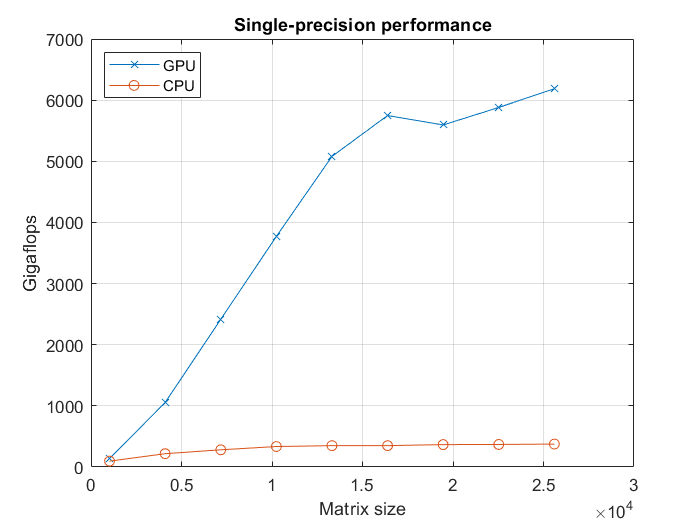
\includegraphics[width=\linewidth]{Figures/Imagenes/single.png}
\caption{}
\end{minipage}
\begin{minipage}[b]{0.32\linewidth}
\centering
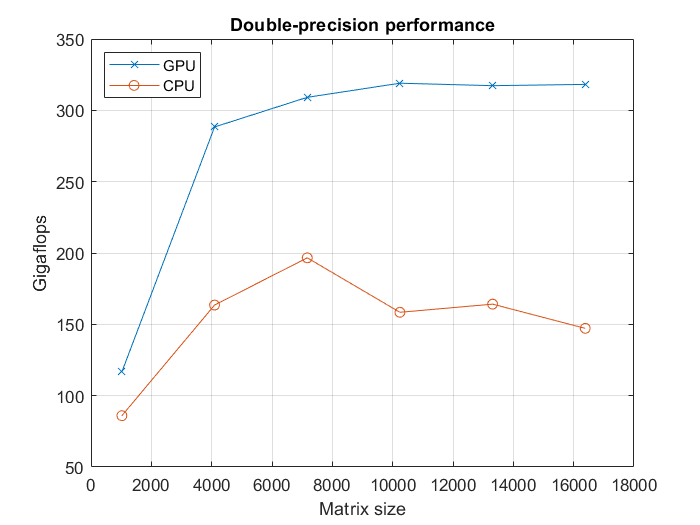
\includegraphics[width=\linewidth]{Figures/Imagenes/double.png}
\caption{}
\end{minipage}
\begin{minipage}[b]{0.32\linewidth}
\centering
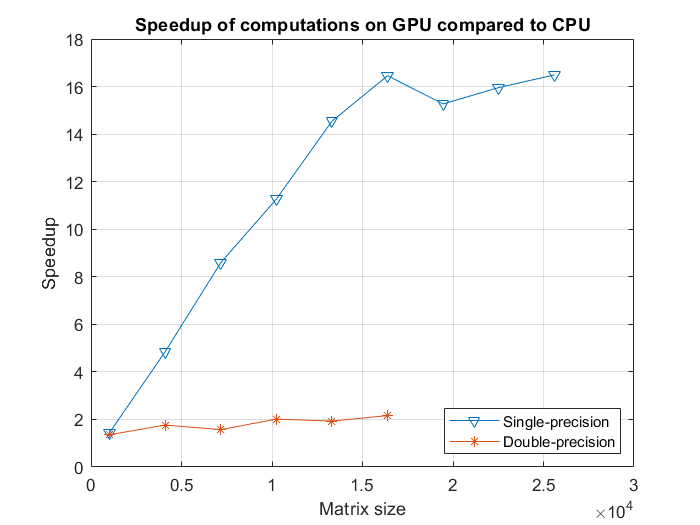
\includegraphics[width=\linewidth]{Figures/Imagenes/speedup.png}
\caption{}
\end{minipage}
\end{figure}
\end{center}

\vspace{-1em}

We can observe that performance under single precision (Figure 1) skyrockets when we use the GPU versus the CPU, we see this is not the case for double precision (Figure 2). In Figure 3, we see a relationship between the performance achieved with the GPU vs. the CPU where we see that the larger the matrix dimension, this ratio increases, seeing results up to 16 times better with the GPU than with the CPU.



\subsection{Python Benchmark (CuPy) code}

To begin with, this first week I will be creating a script of a benchmark for CuPy, comparing its performance to NumPy in the context of matrix-vector multiplication operations. 
We can see the code of the operations below:

\begin{lstlisting}
    print("\nComparing performance for dimension N = {}\n".format(dim))
    
    np_matrix = np.empty((dim, dim), dtype=np.float32)
    np_vector = np.empty(dim, dtype=np.float32)
    numpy_random_matrix(dim, np_matrix)
    numpy_random_vector(dim, np_vector)
    
    start = time.time()
    for i in range(10000):
    
         numpy_result = i*numpy_dot(np_matrix, np_vector)

    numpy_time = time.time() - start


    cp_matrix = cp.empty((dim, dim), dtype=cp.float32)
    cp_vector = cp.empty(dim, dtype=cp.float32)
    cupy_random_matrix(dim, cp_matrix)
    cupy_random_vector(dim, cp_vector)

    start = time.time()
    for i in range(10000):

        cupy_result = i*cupy_dot(cp_matrix, cp_vector)
   
    cupy_time = time.time() - start

    start = time.time()

    np_cupy_result = cp.asnumpy(cupy_result)
    cupy_transfer_time = time.time() - start
    
\end{lstlisting}

\subsection{Why we don't get any better than 15x-20x performance with the GPU}


Modern x86-64 Intel/AMD processor can generally compute 2 (256 AVX) SIMD vectors in parallel since there is generally 2 SIMD units. Processors like Intel Skylake also have 4 ALU units capable of computing 4 basic arithmetic operations (eg. add, sub, and, xor) in parallel per cycle. This can significantly speed up certain operations, especially in tasks like image processing and game physics where the same operations often need to be performed on large sets of data.


To illustrate this comparison further, we can look at the AMD Ryzen 5 5600X CPU. This 6-core processor has 2x256 bit SIMD units per core. This CPU can manage instructions with up to a 512 bit vector as we said before.

\clearpage

However, NVIDIA GPUs execute groups of threads known as warps in SIMT (Single Instruction, Multiple Thread) fashion. In this case, one instruction can operate 32 items in parallel (Remeber, this is theoretically, hardware can be free not to do that completely in parallel). Knowing this, we can consider a CPU core equivalent to ``16 CUDA cores'' (512/32 = 16). Therefore, a Ryzen 5 5600X would have the equivalent to $6 \cdot 16 = 96$ ``CUDA cores''.

We also computed the ratio of the number of CUDA cores in the RTX 3070 (5,888 CUDA cores) to the number of ``CUDA cores'' in the Ryzen 5 5600X:

\vspace{-0.5em}
\begin{center}
$\dfrac{{5888}}{{96}} = 61.33$
\end{center}

This indicates that the GPU has approximately 61.33 times as many CUDA cores as the CPU.

However, we must also consider the clock speeds of the GPU and CPU, which are 1.4 GHz and 4.6 GHz, respectively. Taking this into account, we find that the potential speedup of the GPU compared to the CPU is approximately:

\begin{center}
$\dfrac{{61.33 * 1.4}}{{4.6}} \approx 18.58$.
\end{center}

It's important to understand that these comparisons greatly oversimplify the architectural differences between CPUs and GPUs. They are mainly illustrative and should not be used to predict performance across different types of tasks.


\clearpage

\subsection{Benchmarks repository v1}

Our goal for this week is to create a benchmark repository for Python, Fortran, C, and Matlab. The purpose of this benchmark repository is to compare the execution time of the same operation across these different programming languages.

To recap, in week 1, we performed a particular operation in Python. This week, we will replicate that operation in Fortran, C, and Matlab. By doing so, we can measure and compare the time it takes for each language to perform the same task. This will provide us with useful insights into the relative performance of these languages.

\vspace{1em}


\begin{table}[h]
\resizebox{\textwidth}{!}{%
\begin{tabular}{|c|c|c|c|c|c|c|}
\hline
N                      & \textbf{CPU}              & \textbf{GPU}              & \textbf{Test} & \textbf{CPU (SC) Time} & \textbf{CPU (MC) Time} & \textbf{GPU Time} \\ \hline
\multirow{4}{*}{5000}  & \multirow{4}{*}{R5 5600X} & \multirow{4}{*}{RTX 3070} & Matlab        & 289.03s                & 181.21s                & 8.28s             \\ \cline{4-7} 
                       &                           &                           & Python        & NA                     & 26.41s                 & 2.45s             \\ \cline{4-7} 
                       &                           &                           & Fortran       &                        &                        &                   \\ \cline{4-7} 
                       &                           &                           & C++           & 767.82s                & 101.73s                 &                   \\ \hline
\multirow{4}{*}{10000} & \multirow{4}{*}{R5 5600X} & \multirow{4}{*}{RTX 3070} & Matlab        & 1087.51s               & 637.95s                & 30.24s            \\ \cline{4-7} 
                       &                           &                           & Python        & NA                     & 162.15s                & 9.52s             \\ \cline{4-7} 
                       &                           &                           & Fortran       &                        &                        &                   \\ \cline{4-7} 
                       &                           &                           & C++           &                        &                        &                   \\ \hline
\end{tabular}%
}
\end{table}


Remember that this is a preliminary approach and our first contact with the benchmarks. It serves as a starting point for identifying areas of improvement.


\subsection{Optimizing CPU Utilization with Vectorization}

In light of the performance issues experienced in our single-core benchmarks, our primary focus this week is shifting from GPU parallelization to optimizing CPU utilization. In particular, we will be forcing vectorization to take advantage of SIMD (Single Instruction, Multiple Data) instructions and standards such as AVX2/256bits on my Ryzen 5 5600X

As we have observed from the benchmark test results, in some laguages we are not using 100\% of CPU capacity. One potential reason could be the lack of vectorization in our code. Vectorization is a critical aspect of numerical computation which allows a processor to perform a single operation on multiple data points simultaneously. This can significantly improve the execution speed of our programs.

\clearpage

\subsection{Vectorization in Different Programming Languages}

\subsubsection*{Matlab}
Matlab is inherently good at vectorized operations due to its matrix-based design. It will automatically use vectorization when possible. This is why we got great results without doing any tweak. This was our goal with the rest of languages.

\subsubsection*{Python:} Python, with libraries such as NumPy, can perform vectorized operations efficiently. NumPy arrays can significantly speed up the operations by implicitly allowing element-wise operations. Vectorization here is implicit and does not require any special syntax to enable it. This is due to NumPy's design to handle array operations efficiently by performing element-wise operations on arrays.

However, to ensure that you are taking advantage of vectorization, you should:

\begin{itemize}[label={\scriptsize\raisebox{0.5ex}{\textbullet}}]

\itemsep=0.3em\topsep=0pt\partopsep=0pt
\parskip=0pt\parsep=0pt

\setitemize{leftmargin=1em}

 \item \textbf{Use NumPy's built-in functions} and operations as is optimized for array operations.

 \item \textbf{Avoid loops:} The whole point of vectorization is to eliminate explicit loops over elements in arrays.fhere may be a way to do the operation using NumPy's vectorized operations.

 \item \textbf{Broadcasting:} Understand and utilize broadcasting, a powerful mechanism that allows NumPy to work with arrays of different shapes when performing arithmetic operations. For example, you can add a scalar to an array, and NumPy will add that scalar to each element in the array.
 
\end{itemize}


\subsubsection*{Fortran:}

Intel Fortran have features for automatic vectorization. This includes the use of Single Instruction, Multiple Data (SIMD) instructions.

The Intel Fortran compiler uses various flags to enable and optimize vectorization. For instance, the \texttt{-O3} flag turns on the compiler's optimization, including vectorization.

To benefit the most from vectorization, Fortran code might need adjustments to conform to certain conditions. Some best practices include:

\begin{itemize}
\item \textbf{Loop Independence:} Each iteration of the loop should be independent; the result of an iteration should not depend on the results of other iterations.
\item \textbf{Array Operations:} Fortran naturally lends itself to array operations, which can be implicitly vectorized.
\item \textbf{Compiler Directives:} Compiler directives, such as \texttt{!DIR\$ SIMD} before a loop, can give the compiler hints to assist with vectorization.
\end{itemize}



\subsubsection*{C++:}

The Intel C++ compiler utilizes various flags to enable and guide the process of vectorization. For instance, the \texttt{-O3} flag activates the compiler's optimization, including vectorization. Furthermore, the \texttt{-xHost} flag generates instructions for the highest instruction set available on the host processor. The \texttt{-vec-report} flag can be used to get a report on vectorization decisions made by the compiler.

To fully exploit vectorization, C++ code might need to be adjusted to certain conditions:

\begin{itemize}
\item \textbf{Loop Independence:} The iterations of a loop should ideally be independent; the result of one iteration should not depend on the result of other iterations.
\item \textbf{Data Alignment:} Data should be aligned in memory for optimal performance. Many modern compilers can automatically align data, but it is possible to manually specify alignment in your C++ code.
\item \textbf{Compiler Directives:} Compiler directives or pragmas can provide additional hints to the compiler. For instance, the \texttt{\#pragma simd} directive can suggest to the compiler that a loop should be vectorized.
\end{itemize}

It is important to remember that efficient vectorization requires a deep understanding of the code and the target hardware. Always ensure the correctness of the computation after vectorization, as parallel execution can introduce numerical differences due to the reordering of operations.
\clearpage

\section{Month 2 - June}

\subsection{RAM speed, latency, and system cache}

Different RAM configurations result in different data access times, which could substantially influence the performance of large-scale computations. Generally, operations that involve a high volume of data access can be impacted by RAM speed and latency. We can see here the estimated latency for different RAM configurations:

\vspace{-1.5em}
\begin{equation*}
\begin{split}
    \text{Memory 3200 MHz, CL16:} & \quad \frac{16}{3200} \times 1000 \approx 5 \text{ ms} \\
    \text{Memory 4000 MHz, CL19:} & \quad \frac{19}{4000} \times 1000 \approx 4.75 \text{ ms} \\
    \text{Memory 2400 MHz, CL17:} & \quad \frac{17}{2400} \times 1000 \approx 7.08 \text{ ms} \\
\end{split}
\end{equation*}

Data needs to be fetched frequently from the RAM. If the RAM cannot supply data quickly enough, the CPU might have to wait for the data, leading to a memory bottleneck and a decrease in the overall performance.

In this context, the system's cache is also a key factor. The cache is a smaller, faster type of memory that stores copies of data from frequently used main memory locations. When the CPU needs data, it first looks for it in the cache (starting from L1, then L2, and finally L3). If the data is found there (a cache hit), it can be accessed much faster than from RAM. However, if the data is not in the cache (a cache miss), the CPU has to fetch it from RAM, which takes longer.

The efficiency of cache usage depends on many factors. One of them is data locality – if the data that needs to be accessed is stored close together, it's more likely to be loaded into the cache at the same time, increasing the chances of cache hits in the future. On the contrary, if data is scattered around, loading one piece of data into the cache is less likely to result in future cache hits.

\vspace{0.3em}

\begin{figure}[H]
	\centering
	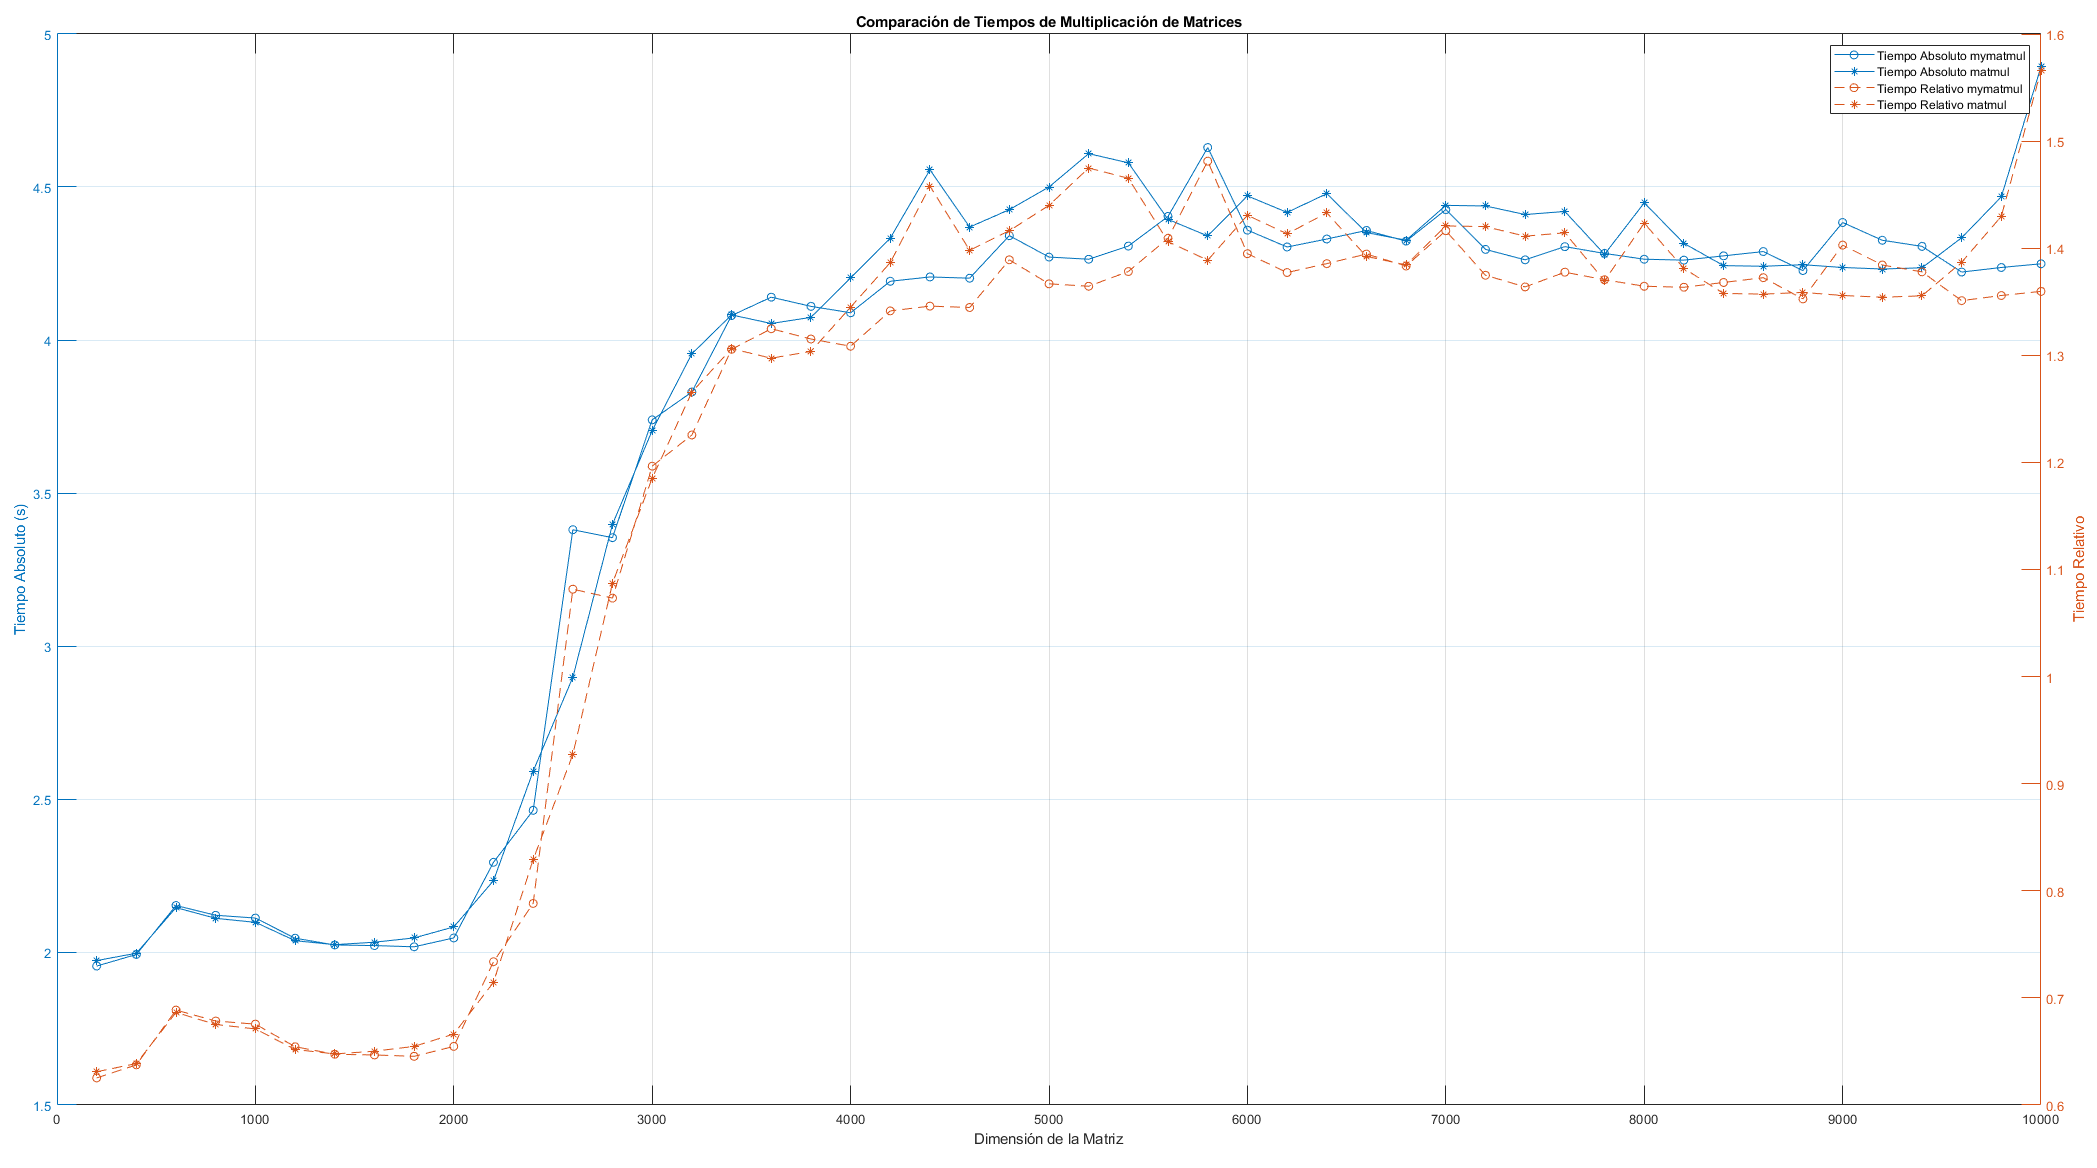
\includegraphics[width=103mm]{Figures/Imagenes/cache_problem.png}
   \caption{Cache memory without a good data locality}
\end{figure}

\clearpage


\subsection{Static vs Dynamic Variables}

When variables are declared as parameters, they are considered constant and occupy a fixed memory location. The Fortran compiler can often perform more aggressive optimizations on these variables since their values don't change at runtime.

Conversely, dynamically allocated variables are more flexible, but this can sometimes lead to less aggressive optimization since the compiler doesn't know the specifics about the memory layout and sizes until runtime.

For performance-critical code, it's generally beneficial to use static variables where possible.

\subsection{512-bit Vector Registers}

Modern CPUs have vector registers that allow for Single Instruction, Multiple Data (SIMD) operations. The 512-bit wide vector registers allow the CPU to perform arithmetic on multiple data points simultaneously, which can significantly speed up operations, especially in the context of matrix computations.

\subsection{Cache Blocking}

As discussed earlier, the processor cache is critical for performance. The cache stores copies of frequently accessed data, allowing the CPU to retrieve it faster compared to main memory. To efficiently utilize the cache, we implemented cache blocking in matrix multiplication. The idea is to divide the matrix into smaller blocks that fit into the cache, reducing the number of cache misses. 

\begin{lstlisting}
integer, parameter :: cacheSize = 32 * 1024 * 1024  ! 32MB
blockSize = int(sqrt(real(cacheSize) / 4.0))

do jj = 1, M, blockSize
    do ii = 1, N, blockSize
        do j = jj, min(jj + blockSize - 1, M)
            do i = ii, min(ii + blockSize - 1, N)
                b(i) = b(i) + A(i, j) * x(j)
            end do
        end do
    end do
end do
\end{lstlisting}


However, it is important to note that cache blocking alone still performs the matrix multiplication sequentially. This means that it only uses a single core of the CPU. In fact, using a single-threaded approach with cache blocking can sometimes result in worse performance compared to a simple matrix multiplication due to the additional loops and steps involved in handling the blocks. Therefore, while cache blocking is an essential optimization technique for reducing cache misses, the performance might still be suboptimal if the computation is not parallelized to take advantage of multiple cores.

\subsection{Thread vs Core Parallelism}

Threads are the smallest unit of processing that can be scheduled by an operating system. Core-level parallelism, on the other hand, refers to executing multiple tasks simultaneously on different physical cores of a processor.

Using threads is useful for hiding latency and is good for I/O bound tasks. Core-level parallelism is more suited for CPU-bound tasks, especially if the threads are not sharing data, as this can lead to a nearly linear speed-up.

\subsection{Parallelization with OpenMP}

To further optimize performance and overcome the limitations of the single-threaded approach, we introduced parallelization using OpenMP. This allows the matrix multiplication to be distributed across multiple CPU cores, greatly reducing the overall computation time.

In the code snippet below, we've combined cache blocking with parallelization. However, parallelizing the loops can introduce concurrency issues. One such issue is race conditions, which occur when multiple threads try to access and modify shared data simultaneously. This can lead to unpredictable and incorrect results.

To manage this, OpenMP provides a reduction clause. This clause ensures that each thread gets a private copy of the shared data, and after the threads have finished their computations, the private copies are combined into a single final result.

\begin{lstlisting}
!$omp parallel private(jj, ii, i, j) 
do jj = 1, M, blockSize
    do ii = 1, N, blockSize
        !$omp do reduction(+:b)
        do j = jj, min(jj + blockSize - 1, M)
            do i = ii, min(ii + blockSize - 1, N)
                b(i) = b(i) + A(i, j) * x(j)
            end do
        end do
        !$omp end do
    end do
end do
!$omp end parallel
\end{lstlisting}

\clearpage

Let's break down the code:

\begin{itemize}
    \item The outermost loops iterate over blocks of the matrix (`do jj = 1, M, blockSize` and `do ii = 1, N, blockSize`). 
    
    \item `!\$omp parallel private(jj, ii, i, j)` initiates a parallel region. The variables inside the private clause (`jj, ii, i, j`) are made private to each thread, meaning that each thread gets its own copy of these variables.
    
    \item `!\$omp do reduction(+:b)` indicates the start of the portion of code that should be executed in parallel by different threads. The reduction clause with the `+:b` operation specifies that we are performing a sum into the array `b`, and OpenMP should handle the reduction in a thread-safe way.
    
    \item The innermost loops (`do j = jj, min(jj + blockSize - 1, M)` and `do i = ii, min(ii + blockSize - 1, N)`) perform the actual multiplication and sum for each block. This part is similar to the standard matrix multiplication but operates on small blocks that fit into the cache.
    
    \item `!\$omp end do` and `!\$omp end parallel` mark the end of the parallel section.
\end{itemize}


With these optimizations, including cache blocking combined with parallelization, matrix-vector multiplication can be significantly accelerated, especially for large matrices where cache efficiency and parallel processing make a substantial difference.


\clearpage

\section{Month 3 - July}

\subsection{GEMMs (General Matrix Multiplications)}

General Matrix Multiplication (GEMM) is defined as the operation $C = AB + C$, with $A$ and $B$ as matrix inputs, and $C$ as a pre-existing matrix which is overwritten by the output.

\subsubsection{Math And Memory Bounds}


Matrix $A$ is an $M \times K$ matrix, meaning that it has $M$ rows and $K$ columns. Similarly, $B$ and $C$ are $K \times N$ and $M \times N$ matrices, respectively. The product of $A$ and $B$ has $M \times N$ values, each of which is a dot-product of $K$-element vectors.

Thus, a total of $M \times N \times K$ fused multiply-adds (FMAs) are needed to compute the product. Each FMA is 2 operations, a multiply and an add, so a total of $2 \times M \times N \times K$ FLOPS are required.


\begin{equation}
\text{Arithmetic Intensity} = \frac{\text{number of FLOPS}}{\text{number of byte accesses}} = \frac{2 \times (M \times N \times K)}{2 \times (M \times K + N \times K + M \times N)}
\end{equation}


For example, consider a $M \times N \times K = 5000 \times 5000 \times 5000$ GEMM. The arithmetic intensity can be calculated as:

\begin{equation}
\text{Arithmetic Intensity} = \frac{2 \times 5000 \times 5000 \times 5000}{2 \times (5000 \times 5000 + 5000 \times 5000 + 5000 \times 5000)} = 1666.67
\end{equation}

\textit{Bytes per FLOP (B/F) is a measurement of memory intensity per compute work or the amount of bytes required to be transferred between the execution unit and the off-chip memory relative to the number of floating-point operations required for a particular task.}

The calculated arithmetic intensity can be compared with the FLOPS:byte ratio to determine if the operation is memory or math limited. For example, the NVIDIA V100 GPU, the FLOPS:byte ratio is 138.9 (I couldn't find info for regular CPUs and GPUs as my Ryzen 5600X and my RTX 3070)

In our case, the arithmetic intensity for a $M \times N \times K = 5000 \times 5000 \times 5000$ GEMM is approximately 1666.67 FLOPS/B. This value is higher than the FLOPS:byte ratio of the NVIDIA V100 GPU. Therefore, this operation would be math limited, meaning the speed of the operation is constrained by the speed at which the GPU can perform calculations rather than the speed at which it can access memory.

If we were to decrease the size of the GEMM such that the resulting arithmetic intensity is lower than the FLOPS:byte ratio of the GPU, then the operation would become memory limited. In a memory limited operation, the speed of the operation is constrained by the speed at which the GPU can access memory rather than the speed at which it can perform calculations.

In particular, it follows from this analysis that matrix-vector products (general matrix-vector product or GEMV), where either $M=1$ or $N=1$, are always memory limited; their arithmetic intensity is less than 1.

Our goal is to determine the FLOPS:byte ratio for our various devices, including different types of CPUs and GPUs. This ratio is a key performance characteristic that can help us understand the balance between computational power and memory bandwidth in a given device. By understanding the FLOPS:byte ratio of our devices, we can make informed decisions about how to best utilize our computational resources.

\subsubsection{A Layered Approach to GEMM}
In the general case, GEMM can be systematically decomposed into multiple calls to special cases. These special cases include GEPP, GEMP, and GEPM operations. Each of these operations can be further decomposed into multiple calls to GEBP, GEPB, or GEPDOT kernels.

The idea is that if these three lowest level kernels attain high performance, then the other cases of GEMM will also perform well. This is illustrated in Fig. 5, which shows the path through the decomposition process that always takes the top branch.

By understanding this layered approach to GEMM, we can gain insights into the performance characteristics of different types of matrix multiplication operations and how they relate to each other.

\begin{figure}[H]
\centering
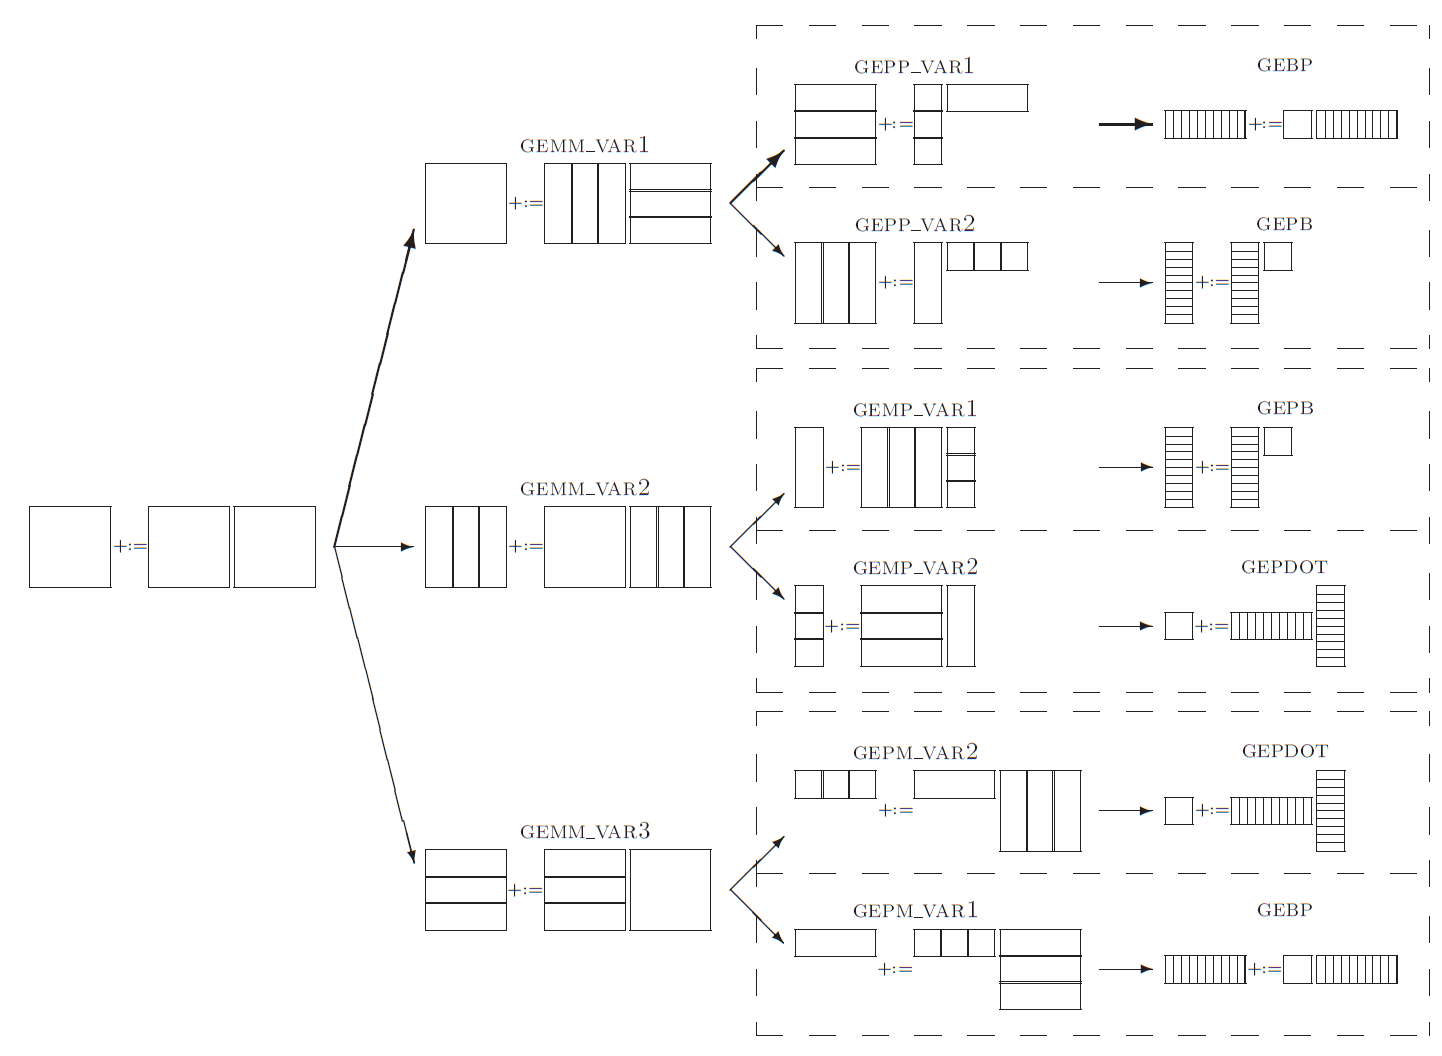
\includegraphics[width=130mm]{Figures/Imagenes/Special_cases_GEMM.png}
\caption{Layered approach to implementing gemm}
\end{figure}

\begin{itemize}
\item \textbf{GEPP (General Matrix-Panel Multiply):} This algorithm performs the multiplication of a general matrix by a panel (a subset of columns) of another matrix. It is useful when one wants to multiply a large matrix by a small submatrix of another matrix.

\item \textbf{GEMP (General Panel-Matrix Multiply):} This is the opposite case to GEPP. It performs the multiplication of a panel (a subset of columns) of a matrix by a general matrix. It is useful when one wants to multiply a small submatrix of a matrix by another large matrix.

\item \textbf{GEPM (General Panel-Panel Multiply):} This algorithm performs the multiplication of a panel (a subset of columns) of a matrix by another panel of another matrix. It is useful when one wants to multiply two small submatrices extracted from larger matrices.
\end{itemize}

As we said, each of these operations can be further decomposed into multiple calls to GEBP, GEPB, or GEPDOT kernels.

\begin{itemize}
\item \textbf{GEBP (General Panel-Block Multiply):} This algorithm performs the multiplication of a panel (a subset of columns) of a matrix by a block (a submatrix) of another matrix. It is useful when one wants to multiply a small submatrix of a matrix by a larger submatrix of another matrix.

\item \textbf{GEPB (General Panel-Block Multiply):} This algorithm performs the multiplication of a panel (a subset of columns) of a matrix by a block (a submatrix) of another matrix. It is useful when one wants to multiply a small submatrix of a matrix by a larger submatrix of another matrix.

\item \textbf{GEPDOT (General Panel-Dot Product):} This algorithm performs the dot product of a panel (a subset of columns) of a matrix with another panel of another matrix. It is useful when one wants to compute the dot product of two small submatrices extracted from larger matrices.
\end{itemize}

\subsubsection*{Cost of moving data between memory layers}
We now discuss techniques for the high-performance implementation of GEBP, GEPB, and GEPDOT. We do so by first analyzing the cost of moving data between memory layers with a naive model of the memory hierarchy. 

\begin{figure}[H]
\centering
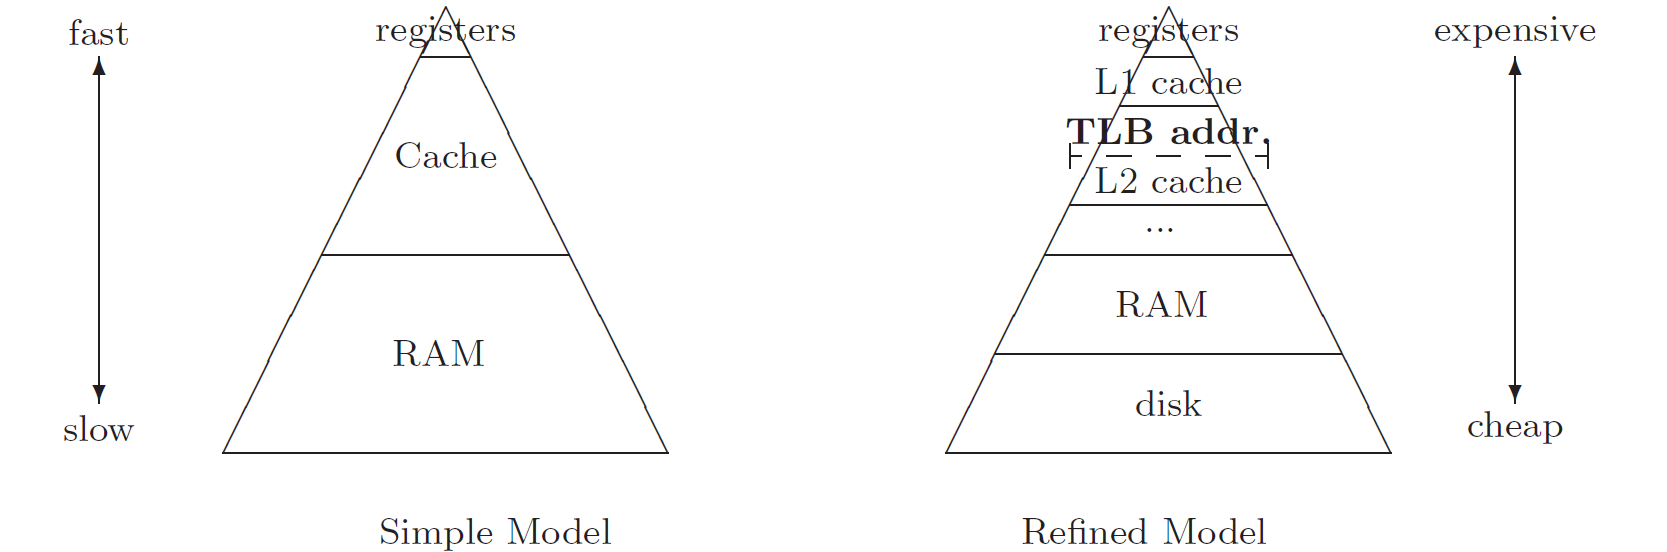
\includegraphics[width=90mm]{Figures/Imagenes/Memory_anatomy.png}
\caption{multi-level cache memory}
\end{figure}

We depict a very simple model of a multi-level cache memory. One layer of cache memory is inserted between the Random-Access Memory (RAM) and the registers. The top-level issues related to the high-performance implementation of GEBP, GEPB, and GEPDOT can be described using this simplified architecture.

\textit{TLB (Translation Lookaside Buffer) is a hardware cache used in processors to accelerate virtual address translation. It stores recently used virtual-to-physical address mappings, reducing the time required for address translation. TLB hits provide fast access to physical addresses, while TLB misses require accessing the page table in memory. TLBs are vital in modern processors for efficient virtual memory systems.}


\begin{figure}[H]
\centering
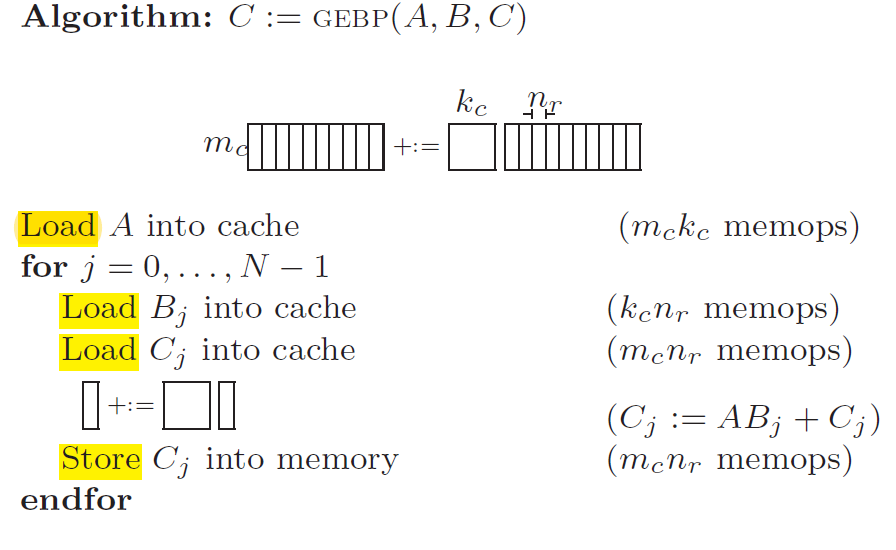
\includegraphics[width=110mm]{Figures/Imagenes/GEBP.png}
\caption{Basic implementation of GEBP}
\end{figure}


Assumption (a): The dimensions $mc$ and $kc$ are small enough so that matrix $A$ and $nr$ columns from each of $B$ and $C$ ($B_j$ and $C_j$, respectively) together fit in the cache.

Assumption (b): If $A$, $C_j$, and $B_j$ are in the cache, then the computation $C_j := AB_j + C_j$ can be performed at the peak rate of the CPU.

Assumption (c): If $A$ is in the cache, it remains there until it is no longer needed.


\clearpage

\subsection{Stack vs Heap}

\begin{itemize}
    \item \textbf{Heap:}
    \begin{enumerate}
        \item Available for the entire program with memory assigned dynamically.
        \item You can decide how much memory to allocate at runtime.
        \item Assigning and deallocating memory from the heap is relatively slow.
        \item In Fortran, global arrays and those allocated with ``allocate()'' are stored in the heap.
    \end{enumerate}

    \item \textbf{Stack:}
    \begin{enumerate}
        \item Has a more limited memory.
        \item Memory allocation and deallocation is very fast.
        \item Local arrays declared in a subroutine are stored in the stack.
        \item Each thread has its own stack.
    \end{enumerate}

    \item \textbf{Interaction between arrays and threads:}
    \begin{enumerate}
        \item All threads share the heap.
        \item If an array in the stack is created inside a parallel region, each thread will have its own copy.
        \item Synchronization is needed if multiple threads want to modify an array in the heap.
    \end{enumerate}

    \item \textbf{Recommendations:}
    \begin{enumerate}
        \item Allocate dynamic arrays only at a high level and infrequently.
        \item Use arrays in the stack for subroutine array temporaries.
        \item Understand the size of these arrays for a good estimation of the necessary stacksize.
    \end{enumerate}
\end{itemize}
\clearpage

\section{Month 4 - August}

\subsection{Optimization module - optimization.f90}
The \texttt{optimization.f90} file integrates a user interface that prompts the user to select from a variety of performance aspects in Fortran. The options available for selection include:

\begin{itemize}[itemsep=0.3ex]
    \item Loop / Array Ordering
    \item Indirect Addressing
    \item Repeated Array Accesses
    \item Array Layout
    \item Array Allocation
    \item Array Slicing
    \item Array Temporaries
    \item Register Spilling
    \item Floating Point Issues
    \item NPROMA Slicing
\end{itemize}

For each of these topics, the program is designed to conduct specific performance tests, demonstrating the practical implications of the respective best practices in real-time Fortran applications. In the subsequent sections, we will present and analyze the results from some of these tests, providing insights into the impact of these practices on computational efficiency and performance.

\paragraph{Reflections on the Optimization Module Results}
From our exploration of the \textit{optimization} module this month, it has become evident that performance optimization in Fortran, while systematic in theory, can yield unpredictable outcomes in practice. While many results align with our expectations, underscoring the value of adhering to best practices, there are instances where the outcomes deviate from the anticipated. Such discrepancies highlight the intricate nature of performance tuning and the myriad of factors that can influence computational efficiency. As we progress in our research, it's imperative to maintain a balance. While the lessons from this module are invaluable, it might be prudent to cease further investigation in areas with diminishing returns and refocus our efforts on core objectives. Nonetheless, the knowledge accrued from this module will undoubtedly shape our future approaches and strategies in Fortran programming.

\clearpage

\subsubsection{Loop Array Ordering}
\textbf{Description:} Loop array ordering deals with the sequence of loops to traverse multi-dimensional arrays. The order can significantly impact cache locality and thus performance. Some results:
\begin{itemize}[itemsep=0.3ex]
    \item \texttt{-Od (nreps=2000)} - Bad: 96.17, Good: 97.1
    \item \texttt{-O1, -O2, -O3 (nreps=2000)} - Bad: N/A, Good: N/A
\end{itemize}

\subsubsection{Indirect Addressing}
\textbf{Description:} Indirect addressing refers to accessing data using pointers or indices, which can sometimes cause the compiler to miss optimization opportunities. Some results:
\begin{itemize}[itemsep=0.3ex]
    \item \texttt{-Od (nreps=20000)} - Bad: 54.27, Good: 57.82
    \item \texttt{-O1 (nreps=20000)} - Bad: 8.01, Good: 11.3
    \item \texttt{-O2 (nreps=20000)} - Bad: 3.157, Good: 3.141
    \item \texttt{-O3 (nreps=20000)} - Bad: 3.163, Good: 3.165
\end{itemize}

\subsubsection{Repeated Array Accesses}
\textbf{Description:} Repeatedly accessing the same array elements can be optimized by storing the elements in temporary variables to reduce access time. Some results:
\begin{itemize}[itemsep=0.3ex]
    \item \texttt{-Od (nreps=20000)} - Bad: 500.5, Good: 484.1
    \item \texttt{-O1, -O2, -O3 (nreps=2000)} - Bad: N/A, Good: N/A
\end{itemize}

\subsubsection{Array Layout}
\textbf{Description:} Array layout optimization aims at arranging data in memory to maximize cache utilization. Some results: 
\begin{itemize}[itemsep=0.3ex]
    \item \texttt{-Od (nreps=2000000)} - Bad: 10.76, Good: 14.38
    \item \texttt{-O1 (nreps=2000000)} - Bad: 6.13, Good: 8.14
    \item \texttt{-O2 (nreps=2000000)} - Bad: 6.13, Good: 8.74
    \item \texttt{-O3 (nreps=2000000)} - Bad: 6.12, Good: 8.13
\end{itemize}

\subsubsection{Array Allocation}
\textbf{Description:} Array Allocation highlights the distinctions between heap and stack memory allocations in Fortran, emphasizing their implications for performance and multithreading.


\subsubsection{Array Slicing}
\textbf{Description:} Array slicing is the practice of taking sub-arrays from an existing array, which can sometimes slow down operations if not done carefully. Some results:
\begin{itemize}[itemsep=0.3ex]
    \item \texttt{-Od (nreps=100000)} - Bad: 522.6, Good: 715.6
    \item \texttt{-O1 (nreps=100000)} - Bad: 109.2, Good: 76.8
    \item \texttt{-O2 (nreps=100000)} - Bad: 17.11, Good: 18.98
    \item \texttt{-O3 (nreps=100000)} - Bad: 17.2, Good: 17.38
\end{itemize}

\subsubsection{Array Temporaries}
\textbf{Description:} Using temporary arrays can sometimes be inefficient as it might require extra memory allocation and data movement.

\subsubsection*{Register Spilling}
\textbf{Description:} Register spilling occurs when there are more active variables than registers, leading to inefficient use of memory. Some results:
\begin{itemize}[itemsep=0.3ex]
    \item \texttt{-Od (nreps=100000000)} - Bad: 17.37, Good: 17.32
    \item \texttt{-O1, -O2, -O3 (nreps=2000)} - Bad: N/A, Good: N/A
\end{itemize}

\subsubsection{Floating Point Issues}
\textbf{Description:} Floating-point arithmetic, like division and exponentiation, can be computationally expensive.

\subsection*{Disclaimer}
While many of these practices theoretically promise improved performance, it's important to note that their practical application can sometimes lead to unexpected outcomes. As observed, certain implementations appear to interfere with, or even negate, the compiler's internal optimizations when activated (showed as N/A in the results).

\clearpage

\section{Month 5 - September}

\subsection*{Back to May}

We took a good look at our optimization module. It was a great learning step, but there might be better ways to push performance. We originally wanted to beat Matlab in speed, and we did it. Now, we're checking which tools can help us improve even more.

We aim to compare the speed-up achieved using multicore versus singlecore on the CPU. Additionally, we'll examine the performance differences between GPU and CPU.

We'll be trying out a few libraries, including Intel MKL, BLIS, and AOCL Blas for the CPU. On the GPU side, we're using \texttt{cupy} to see how it handles the matrix multiplication $C = A \times B$.


\subsection*{Theoretical Limits}
Understanding processors' capabilities is vital for estimating matrix multiplication performance. For matrix multiplication \(C = A \times B\), with matrices of dimension \(N \times N\), repeated \(TIMES\) times, the workload is defined by:
\begin{equation}
    N_{\text{ops}} = 2 \times N^3 \times TIMES
\end{equation}
Matrix multiplication involves a sequence of four operations:
\begin{enumerate}
    \item Accessing values in matrix A
    \item Accessing values in matrix B
    \item Conducting the multiplication
    \item Storing results in matrix C
\end{enumerate}

\subsection{Vectorization}
Vectorization is a fundamental feature inherent to modern processor architectures. It pertains to the execution of operations on extensive data sets, in contrast to singular data elements. Processors equipped with 512-bit registers can process multiple data elements concurrently. This capability allows for optimal use of the processor's computational resources, enhancing the speed of operations. As a result, operations previously restricted to serial execution can now undergo parallel processing, increasing computational efficiency and reducing execution time for data-intensive tasks.

\clearpage

\subsection{Micro-operations}
Micro-operations illustrate a processor's capacity to process multiple tasks within one cycle, enabled by pipelining and throughput techniques.

In the past, first-generation CPUs typically executed fewer than one operation per cycle. In contrast, contemporary pipelined superscalar processors can perform several operations in a single cycle, although this is constrained by specific limits determined by different CPU processing stages.

The micro-operations performance of various processors is tabulated below:

\subsection{Estimating CPU Time}
Based on the above factors, CPU performance can be estimated as:
\begin{equation}
    t_{\text{CPU}} = \frac{4 \times N_{\text{ops}}}{{V_{\text{vectorization}}} \times GHz_{\text{CPU}} \times M_{\text{micro-ops}} \times C_{\text{CPU}}}
\end{equation}

Where the parameters are:
\begin{enumerate}
    \item $V_{\text{vectorization}}$: Vectorization factor: 16 (512-bit)
    \item $M_{\text{micro-ops}}$: Micro-operations factor: 4, 6 (AMD Zen 3) or even 8 (Apple Silicon)
    \item $GHz_{\text{CPU}}$: Clock speed of the CPU
    \item $C_{\text{CPU}}$: Number of cores in the CPU
    \item The factor of 4 accounts for the 4-step sequence in matrix multiplication, as discussed earlier.
\end{enumerate}

\subsection{GPU Time Estimation}
GPUs, having a different architecture, excel in parallelism with a high core count. The estimated operational time for a GPU is:
\begin{equation}
    t_{\text{GPU}} = \frac{N_{\text{ops}}}{GHz_{\text{GPU}} \times C_{\text{GPU}}}
\end{equation}

\subsection{Comparative Analysis: CPU vs GPU}
Comparing CPU and GPU operational speeds, we obtain:
\begin{equation}
    \frac{t_{\text{CPU}}}{t_{\text{GPU}}} = \frac{4 \times GHz_{\text{GPU}} \times C_{\text{GPU}}}{GHz_{\text{CPU}} \times F_{\text{vec}} \times F_{\mu} \times C_{\text{CPU}}}
\end{equation}
It's important to consider that actual performance may vary from these theoretical estimations.


\clearpage

\subsection{Repository of the code and how have been used}

\subsubsection{Fortran - Intel MKL}

The following Fortran code utilizes Intel's Math Kernel Library (MKL). The Intel MKL is a highly optimized, extensively threaded, and thread-safe library of mathematical functions for science, engineering, and financial applications. It's designed to provide maximum performance on a range of Intel processors (We might get worse results because of that, I have an AMD CPU).



\begin{lstlisting}[language=Fortran]
    program C_AxB
    
    use omp_lib

    implicit none
    real, allocatable :: A(:,:), B(:,:), C(:,:)
    real :: power
    integer :: i, unitNum
    integer :: rate, t0, t1
    character(len=250) :: fileName
    integer (kind=8) :: N_ops, N, TIMES
    real :: execution_time
    
    N_ops = 2 * 10000_8**3;
    write(*,*) "CPU TEST RUNNING with N_ops = ", N_ops
    
    ! Loop TIMES(N)
    do N = 25, 2499, 25
        
        TIMES = nint(N_ops / real(2*N**3, 8))
        
        allocate(A(N, N), B(N, N), C(N, N))
        call random_number(A)
        call random_number(B)
        C = 0
        
        call system_clock(t0)
        call system_clock(count_rate=rate)

        !$omp parallel do private(i) % Multicore with OpenMP
        do i = 1, TIMES
            call sgemm("N", "N", N, N, N, 1e0, A, N, B, N, 0, C, N)
        end do
        call system_clock(t1)
        !$omp end parallel do
        
        execution_time = (t1 - t0) / real(rate)
        write(*,*) N, TIMES, execution_time
        deallocate(A, B, C)
        
    end do
    
    
    ! Loop N(TIMES)
    do TIMES = 64, 1, -1
        
        power = 1./3
        N = nint((real(10000_8**3) / TIMES)**power)
        dimensions(TIMES) = N
        
        allocate(A(N, N), B(N, N), C(N, N))
        call random_number(A)
        call random_number(B)
        C = 0
        
        call system_clock(t0)
        call system_clock(count_rate=rate)
        !$omp parallel do private(i) % Multicore with OpenMP
        do i = 1, TIMES
            call sgemm("N", "N", N, N, N, 1e0, A, N, B, N, 0, C, N)
        end do
        !$omp end parallel do
        call system_clock(t1)
        
        execution_time = (t1 - t0) / real(rate)
        write(*,*) n, times, execution_time
        deallocate(A, B, C)
        
    end do
    
    close(unitNum)
    
    end program C_AxB

\end{lstlisting}


\textbf{OpenMP directives:} In this Fortran example utilizing Intel's Math Kernel Library (MKL), the employment or omission of OpenMP directives is pivotal. While the program is inherently optimized for Intel processors, the OpenMP integration provides flexibility. By including or excluding these directives, users can either exploit the full parallel capabilities of their multi-core systems or opt for single-core execution. 

\subsubsection*{Single core:}

\begin{lstlisting}[language=Fortran]
        do i = 1, TIMES
            call sgemm("N", "N", N, N, N, 1e0, A, N, B, N, 0, C, N)
        end do
\end{lstlisting}

\subsubsection*{Multi core:}

\begin{lstlisting}[language=Fortran]
        !$omp parallel do private(i) % Multicore with OpenMP
        do i = 1, TIMES
            call sgemm("N", "N", N, N, N, 1e0, A, N, B, N, 0, C, N)
        end do
        !$omp end parallel do
\end{lstlisting}

\clearpage

\subsubsection{C - BLIS and AOCL}

BLIS (BLAS-like Library Instantiation Software Framework) is a portable \href{https://github.com/flame/blis#how-to-download-blis}{software} framework for instantiating high-performance BLAS-like dense linear algebra libraries. The framework was designed to isolate essential kernels of computation that, when optimized, immediately enable optimized implementations of most of its commonly used and computationally intensive operations.

The AMD Optimized C/C++ \& Fortran Compilers (AOCC) leverage the AMD Zen core microarchitecture. These AOCC compilers provide improved performance on AMD processors, and the same optimizations available in the AOCC compilers are now available in \href{https://github.com/amd/blis}{AMD's fork of BLIS}.

Since AOCL is a fork of BLIS, it utilizes the same set of API calls and functionalities. This means that code written using BLIS functions can be easily ported to make use of AOCL.

\subsection*{Singlecore}
\vspace{-1em}
\begin{lstlisting}[language=C]
#include <stdio.h>
#include <time.h>
#include <math.h>
#include "blis.h"

int main( int argc, char** argv )
{
    FILE *fp;
    num_t dt_r, dt_c;
    dim_t m, n, k;
    inc_t rs, cs;
    long long int N_ops, TIMES;
    double elapsed_time;

    obj_t a, b, c;
    obj_t* alpha;
    obj_t* beta;

    dt_r = BLIS_SINGLE_PREC;
    dt_c = BLIS_SINGLE_PREC;
    rs = 0; cs = 0;
    alpha = &BLIS_ONE;
    beta  = &BLIS_ZERO;
    N_ops = 2 * 10000LL * 10000LL * 10000LL;

    fp = fopen("octubre_blis_single.csv", "w");
    if (!fp) {
        perror("Failed to open file");
        return 1;
    }
    fprintf(fp, "N,TIMES,Execution Time (s)\n");

    for (dim_t dim = 25; dim <= 2499; dim += 25)
    {
        m = n = k = dim;
        TIMES = N_ops / (2LL * m * n * k);

        
        bli_obj_create( dt_c, m, n, rs, cs, &c );
        bli_obj_create( dt_r, m, k, rs, cs, &a );
        bli_obj_create( dt_c, k, n, rs, cs, &b );

        bli_randm( &a );
        bli_randm( &b );
        bli_setm( &BLIS_ZERO, &c );

        clock_t start = clock();
        for (long long int i = 0; i < TIMES; i++)
        {
            bli_gemm( alpha, &a, &b, beta, &c );
        }

        clock_t end = clock();
        elapsed_time = (double)(end - start) / CLOCKS_PER_SEC;

        fprintf(fp, "%ld,%lld,%f\n", dim, TIMES, elapsed_time);
        printf("%lld,%lld,%f\n", dim, TIMES, elapsed_time);

        bli_obj_free( &a );
        bli_obj_free( &b );
        bli_obj_free( &c );
    }

    for (long long int TIMES = 64; TIMES >= 1; TIMES--)
    {
        double power = 1.0 / 3.0;
        long long int N = (long long int) round(pow((double)(10000LL * 10000LL * 10000LL) / TIMES, power));

        m = n = k = N;

        bli_obj_create(dt_c, m, n, rs, cs, &c);
        bli_obj_create(dt_r, m, k, rs, cs, &a);
        bli_obj_create(dt_c, k, n, rs, cs, &b);

        bli_randm(&a);
        bli_randm(&b);
        bli_setm(&BLIS_ZERO, &c);

        clock_t start = clock();
        for (long long int i = 0; i < TIMES; i++)
        {
            bli_gemm(alpha, &a, &b, beta, &c);
        }

        clock_t end = clock();
        double elapsed_time = (double)(end - start) / CLOCKS_PER_SEC;

        fprintf(fp, "%lld,%lld,%f\n", N, TIMES, elapsed_time);
        printf("%lld,%lld,%f\n", N, TIMES, elapsed_time);

        bli_obj_free(&a);
        bli_obj_free(&b);
        bli_obj_free(&c);
    }

    fclose(fp);
    return 0;
}
\end{lstlisting}


\subsection*{Multicore}


\begin{lstlisting}[language=C]
#include <stdio.h>
#include <math.h>
#include <omp.h>
#include "blis.h"

int main( int argc, char** argv )
{
    FILE *fp;
    num_t dt_r, dt_c;
    dim_t m, n, k;
    inc_t rs, cs;
    long long int N_ops, TIMES;
    double elapsed_time;

    obj_t a, b, c;
    obj_t* alpha;
    obj_t* beta;

    dt_r = BLIS_SINGLE_PREC;
    dt_c = BLIS_SINGLE_PREC;
    rs = 0; cs = 0;
    alpha = &BLIS_ONE;
    beta  = &BLIS_ZERO;
    N_ops = 2 * 10000LL * 10000LL * 10000LL;

    fp = fopen("octubre_aocl_multi.csv", "w");
    if (!fp) {
        perror("Failed to open file");
        return 1;
    }
    fprintf(fp, "N,TIMES,Execution Time (s)\n");

    for (dim_t dim = 25; dim <= 2499; dim += 25)
    {
        m = n = k = dim;
        TIMES = N_ops / (2LL * m * n * k);

        bli_obj_create( dt_c, m, n, rs, cs, &c );
        bli_obj_create( dt_r, m, k, rs, cs, &a );
        bli_obj_create( dt_c, k, n, rs, cs, &b );

        bli_randm( &a );
        bli_randm( &b );
        bli_setm( &BLIS_ZERO, &c );

        double start = omp_get_wtime();

        #pragma omp parallel for
        for (long long int i = 0; i < TIMES; i++)
        {
            bli_gemm( alpha, &a, &b, beta, &c );
        }

        double end = omp_get_wtime();
        elapsed_time = end - start;

        fprintf(fp, "%lld,%lld,%.10f\n", dim, TIMES, elapsed_time);
        printf("%lld,%lld,%.10f\n", dim, TIMES, elapsed_time);

        bli_obj_free( &a );
        bli_obj_free( &b );
        bli_obj_free( &c );
    }

    for (long long int TIMES = 64; TIMES >= 1; TIMES--)
    {
        double power = 1.0 / 3.0;
        long long int N = (long long int) round(pow((double)(10000LL * 10000LL * 10000LL) / TIMES, power));

        m = n = k = N;

        bli_obj_create(dt_c, m, n, rs, cs, &c);
        bli_obj_create(dt_r, m, k, rs, cs, &a);
        bli_obj_create(dt_c, k, n, rs, cs, &b);

        bli_randm(&a);
        bli_randm(&b);
        bli_setm(&BLIS_ZERO, &c);

        double start = omp_get_wtime();

        #pragma omp parallel for
        for (long long int i = 0; i < TIMES; i++)
        {
            bli_gemm(alpha, &a, &b, beta, &c);
        }

        double end = omp_get_wtime();
        elapsed_time = end - start;

        fprintf(fp, "%lld,%lld,%.10f\n", N, TIMES, elapsed_time);
        printf("%lld,%lld,%.10f\n", N, TIMES, elapsed_time);

        bli_obj_free(&a);
        bli_obj_free(&b);
        bli_obj_free(&c);
    }

    fclose(fp);
    return 0;
}
\end{lstlisting}

Both the following terminal commands reveals the shared nature of the AOCL and BLIS libraries:

\begin{lstlisting}[language=bash]
gcc gemm.c -I/.../AOCL_folder/blis/include/zen3/ -L/usr/local/lib/libblis.so -lblis -lm -lpthread -o gemm.x
\end{lstlisting}

\begin{lstlisting}[language=bash]
gcc gemm.c -I/.../BLIS_folder/blis/include/zen3/ -L/usr/local/lib/libblis.so -lblis -lm -lpthread -o gemm.x
\end{lstlisting}

The AOCL, being a fork of BLIS, originates from the BLIS codebase, making their APIs and functionalities align closely. For multicore, you need to add the \texttt{-fopenmp} flag.


\subsubsection{Python - CuPy}

CuPy is an open-source matrix library that leverages the computational power of Graphics Processing Units (GPUs) to deliver accelerated performance for array operations. Comparable to NumPy, a well-established array library in Python, CuPy offers a multidimensional array and mathematical functions with a similar use.

The primary advantage of CuPy is its ability to directly use CUDA-native memory and algorithms.

\begin{lstlisting}[language=Python]
import csv
import cupy as cp
import numpy as np

def ab_multiply(C, A, B, TIMES):
    for _ in range(TIMES):
        C[:] = cp.dot(A, B)  # gemm on GPU
        C_cpu = cp.asnumpy(C) # Transferencia de C de la GPU a la memoria principal

def perform_computation_and_record_time(N, TIMES):
    print(N)
    A = cp.random.rand(N, N).astype(cp.float32)
    B = cp.random.rand(N, N).astype(cp.float32)
    C = cp.empty((N, N))
    
    start_event = cp.cuda.Event()
    end_event = cp.cuda.Event()
    start_event.record()
    ab_multiply(C, A, B, TIMES)
    end_event.record()
    end_event.synchronize()

    elapsed_time = cp.cuda.get_elapsed_time(start_event, end_event)
    computation_times.append(elapsed_time)
    N_list.append(N)
   
N_ops = 2 * 10000**3
computation_times = []
N_list = []

# TIMES(N) loop
for N in range(250, 2499, 25):
    TIMES = int(np.ceil(N_ops / (2 * N**3)))
    perform_computation_and_record_time(N, TIMES)

# N(TIMES) loop
for TIMES in range(64, 0, -1):
    N = round((N_ops / (2.0 * TIMES)) ** (1./3))
    perform_computation_and_record_time(N, TIMES)



# Write results to CSV
with open(
    "Resultados/results_octubre_gpu_nomem.csv", mode="w", newline="", encoding="utf-8"
) as file:
    writer = csv.writer(file)
    writer.writerows(zip(N_list, computation_times))
\end{lstlisting}
\section{Final results}

\subsection{Absolute Execution Times}

The first graph illustrates the absolute execution time for the MKL, BLIS, and AOCL implementations, in both single-core and multi-core modes.

\begin{figure}[h!] % [h!] forces the figure to appear here
    \centering
    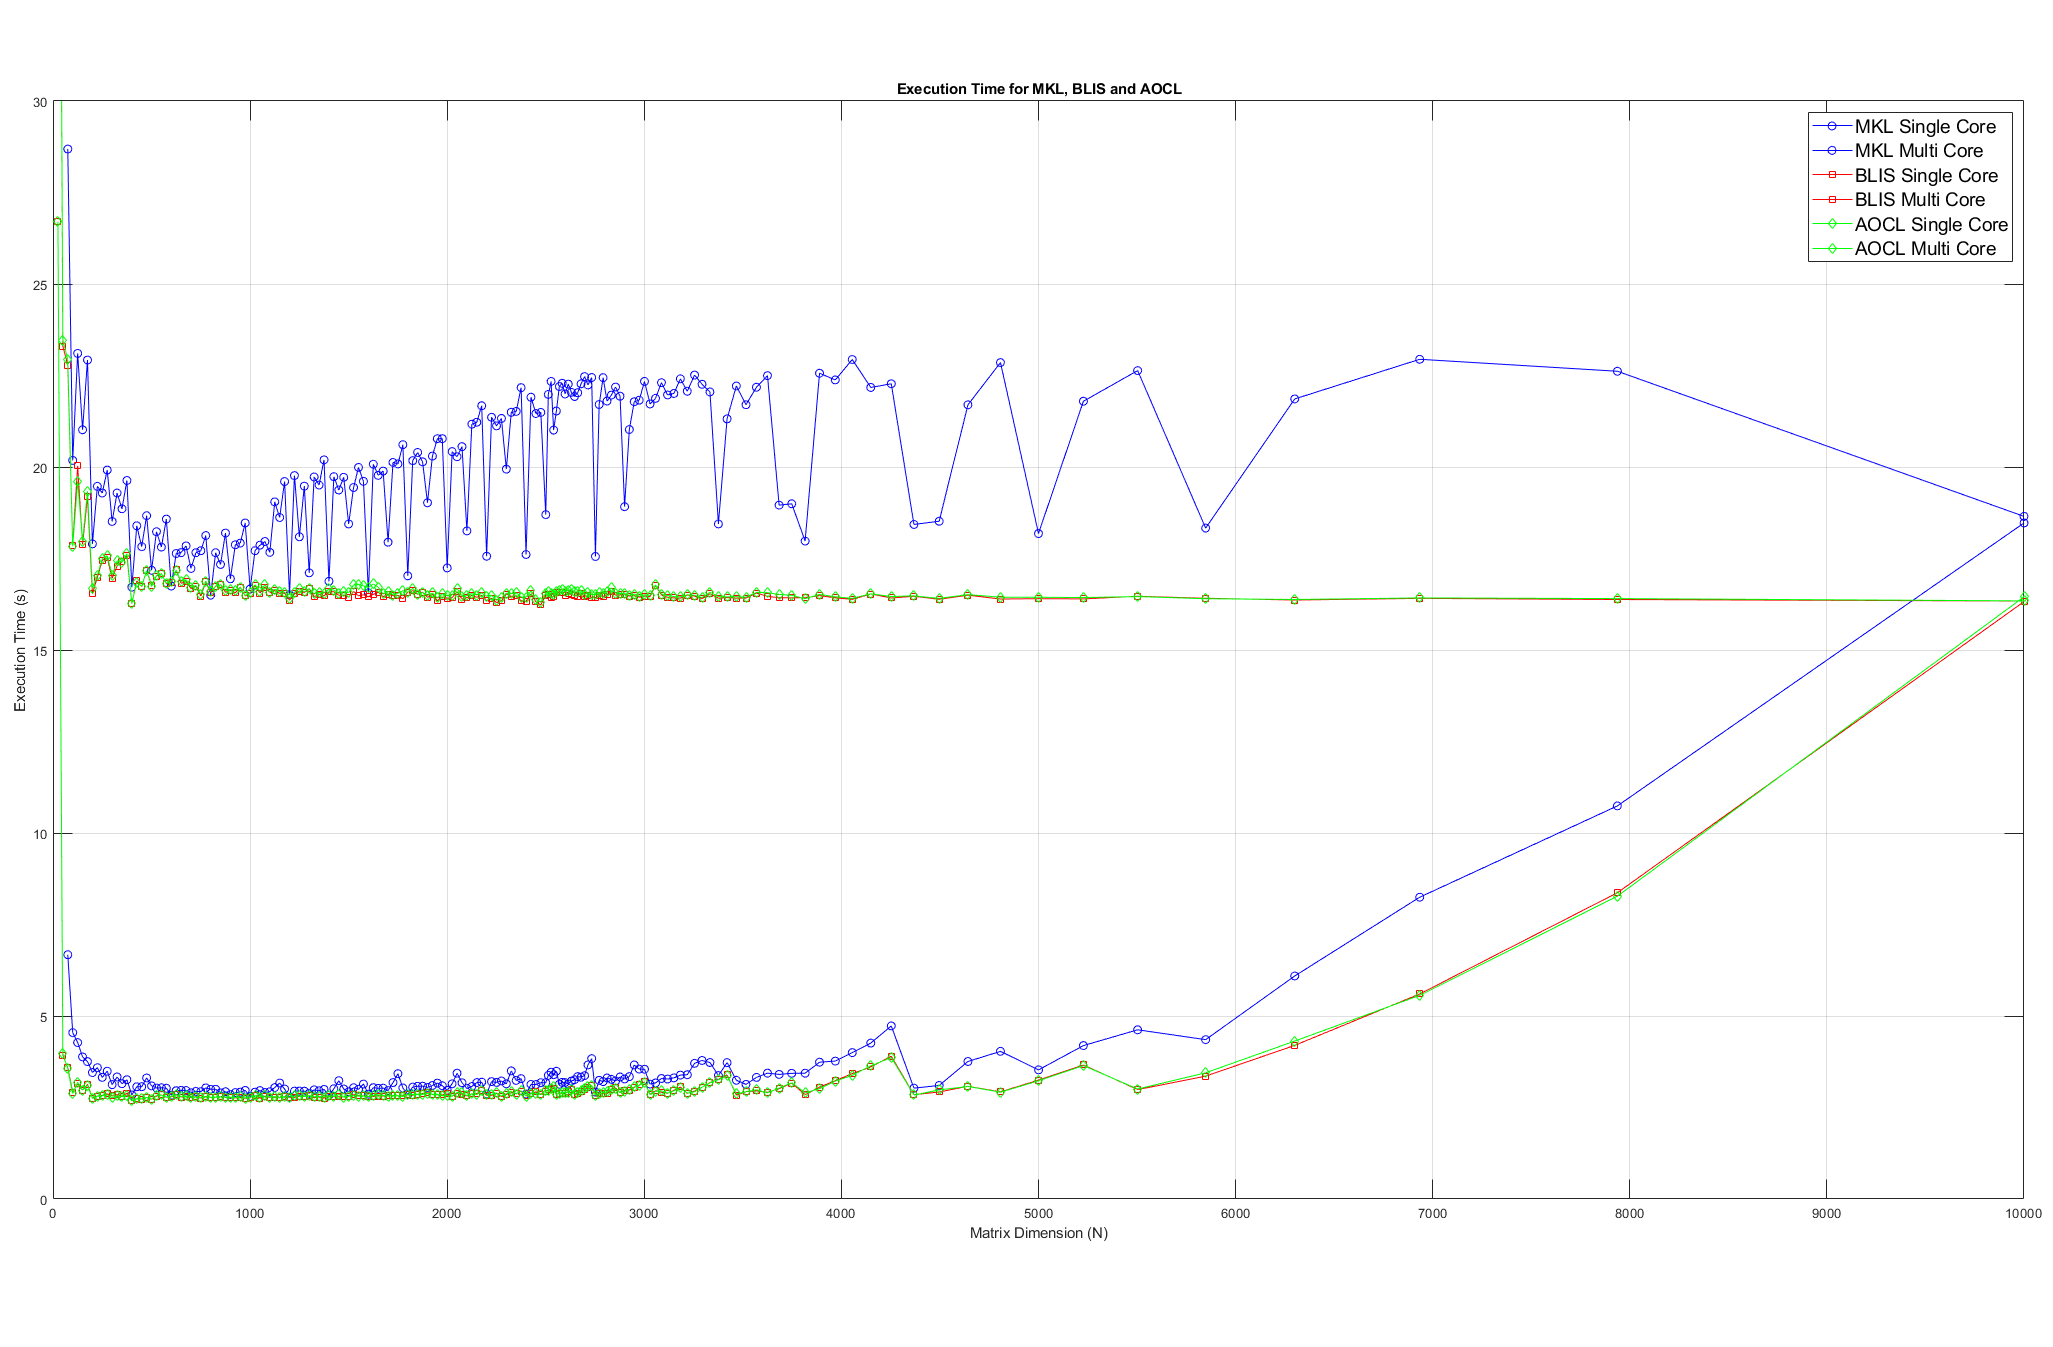
\includegraphics[width=\linewidth]{Figures/Imagenes/Final1.png} % Adjusts the image to the width of the line
    \caption{}
\end{figure}

\begin{itemize}
    \item \textbf{MKL:} Intel's MKL library, while known for its performance on Intel processors, delivered unexpected results on the AMD Ryzen 5 5600X. The single-core performance, in particular, displayed anomalies. One plausible reason could be the library's optimization towards Intel architectures, which might not translate as effectively on AMD platforms. However, its multi-core capability does show some improvement.
    
    \item \textbf{BLIS:} BLIS showcased a consistent performance across both single-core and multi-core modes. Its execution times provide a stable benchmark, demonstrating adaptability across different processor architectures.
    
    \item \textbf{AOCL:} Given that AOCL is a fork of BLIS, their results mirroring each other was expected. This matching performance in both single-core and multi-core modes underscores AOCL's roots in the BLIS codebase.
\end{itemize}



\subsection{Speed Up: Comparison of Single Core vs Multi Core}

The speed-up factor reflects the efficiency with which each implementation harnesses parallelism when activating multiple cores. The second graph underscores the intricacies of the interplay between single-core anomalies and perceived multi-core speed-up benefits.

\begin{figure}[h!] % [h!] forces the figure to appear here
    \centering
    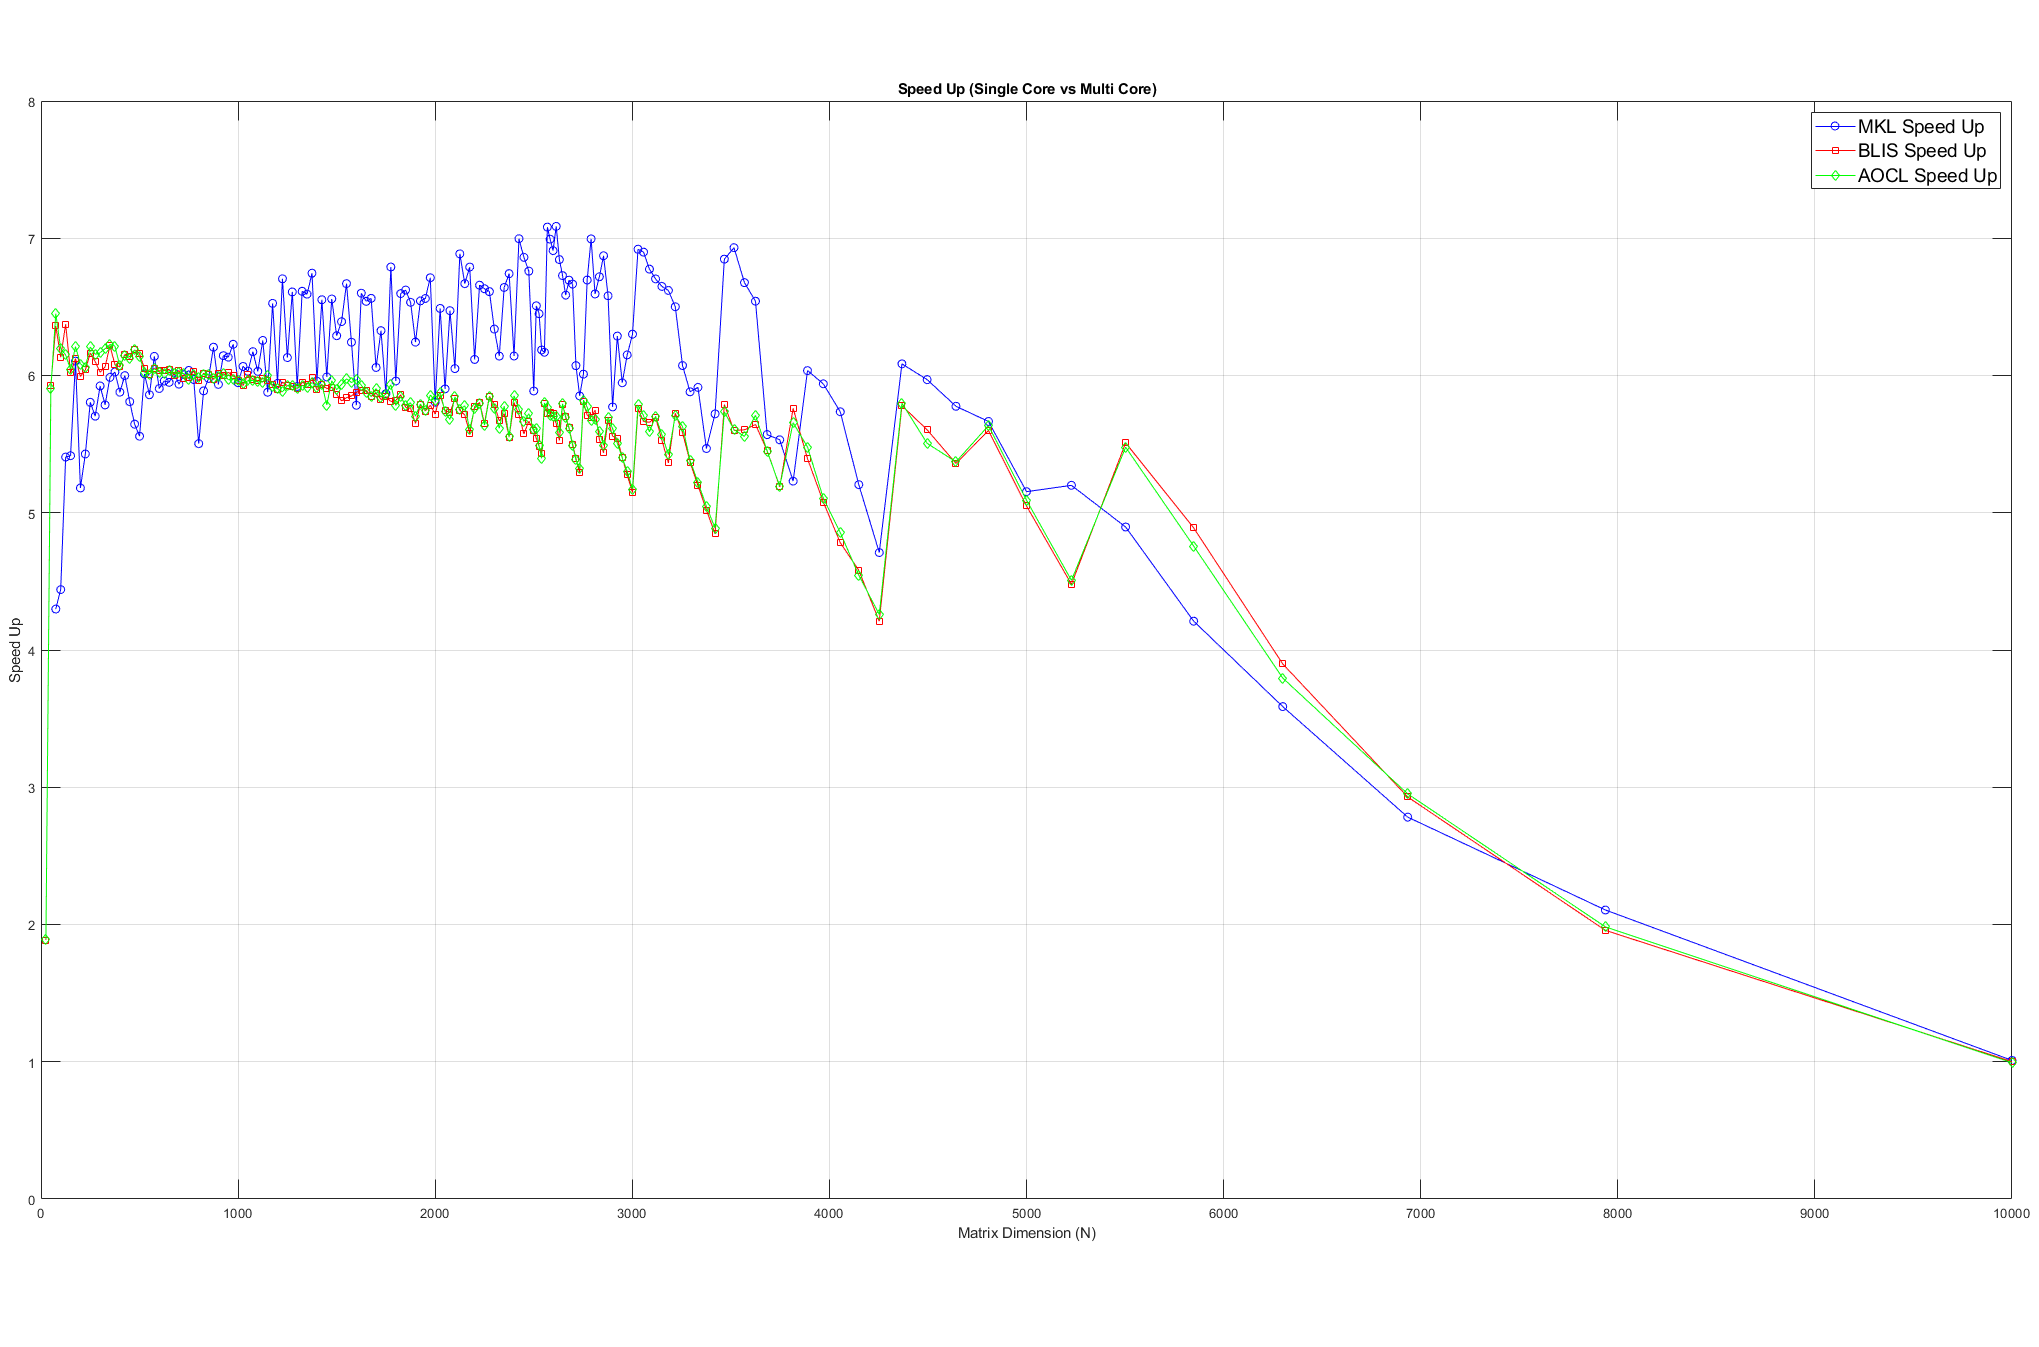
\includegraphics[width=\linewidth]{Figures/Imagenes/Final2.png} % Adjusts the image to the width of the line
\end{figure}
\vspace{-1em}
\begin{itemize}
    \item \textbf{MKL:} With the unexpected behavior in single-core performance already commented, MKL seems to present an exaggerated speed-up, surpassing theoretical limits. This is misleading, as the poor single-core performance artificially boosts the speed-up metric when transitioning to multi-core. Maximum speed-up would be 6, given the AMD Ryzen 5 5600X's 6 cores.
    
    \item \textbf{BLIS and AOCL:} Both BLIS and AOCL showcase a more uniform behavior, aligned with anticipated speed-ups on a 6-core processor. However, as the matrix dimension \( N \) increases, there's a notable decline in the speed-up. This reduction is largely due to the operation loop running over the variable \texttt{TIMES}. As \( N \) grows, \texttt{TIMES} diminishes to maintain a consistent operation count. When \texttt{TIMES} drops below the number of cores, some cores remain idle during the multi-core test, as there isn't enough work to parallelize across all cores. This is particularly evident with \( N=10000 \) where the speed-up approaches 1, indicating that only a single core is actively computing.

\end{itemize}


\subsection{Final Comparison of Execution Times}

The graph below contrasts the execution times of multi-core CPU and GPU matrix computations. GPU tests were made with and without the data transfer between GPU and CPU (the memory transfer is set for every operation, being the worst case scenario possible).

\begin{figure}[h!] % [h!] forces the figure to appear here
    \centering
    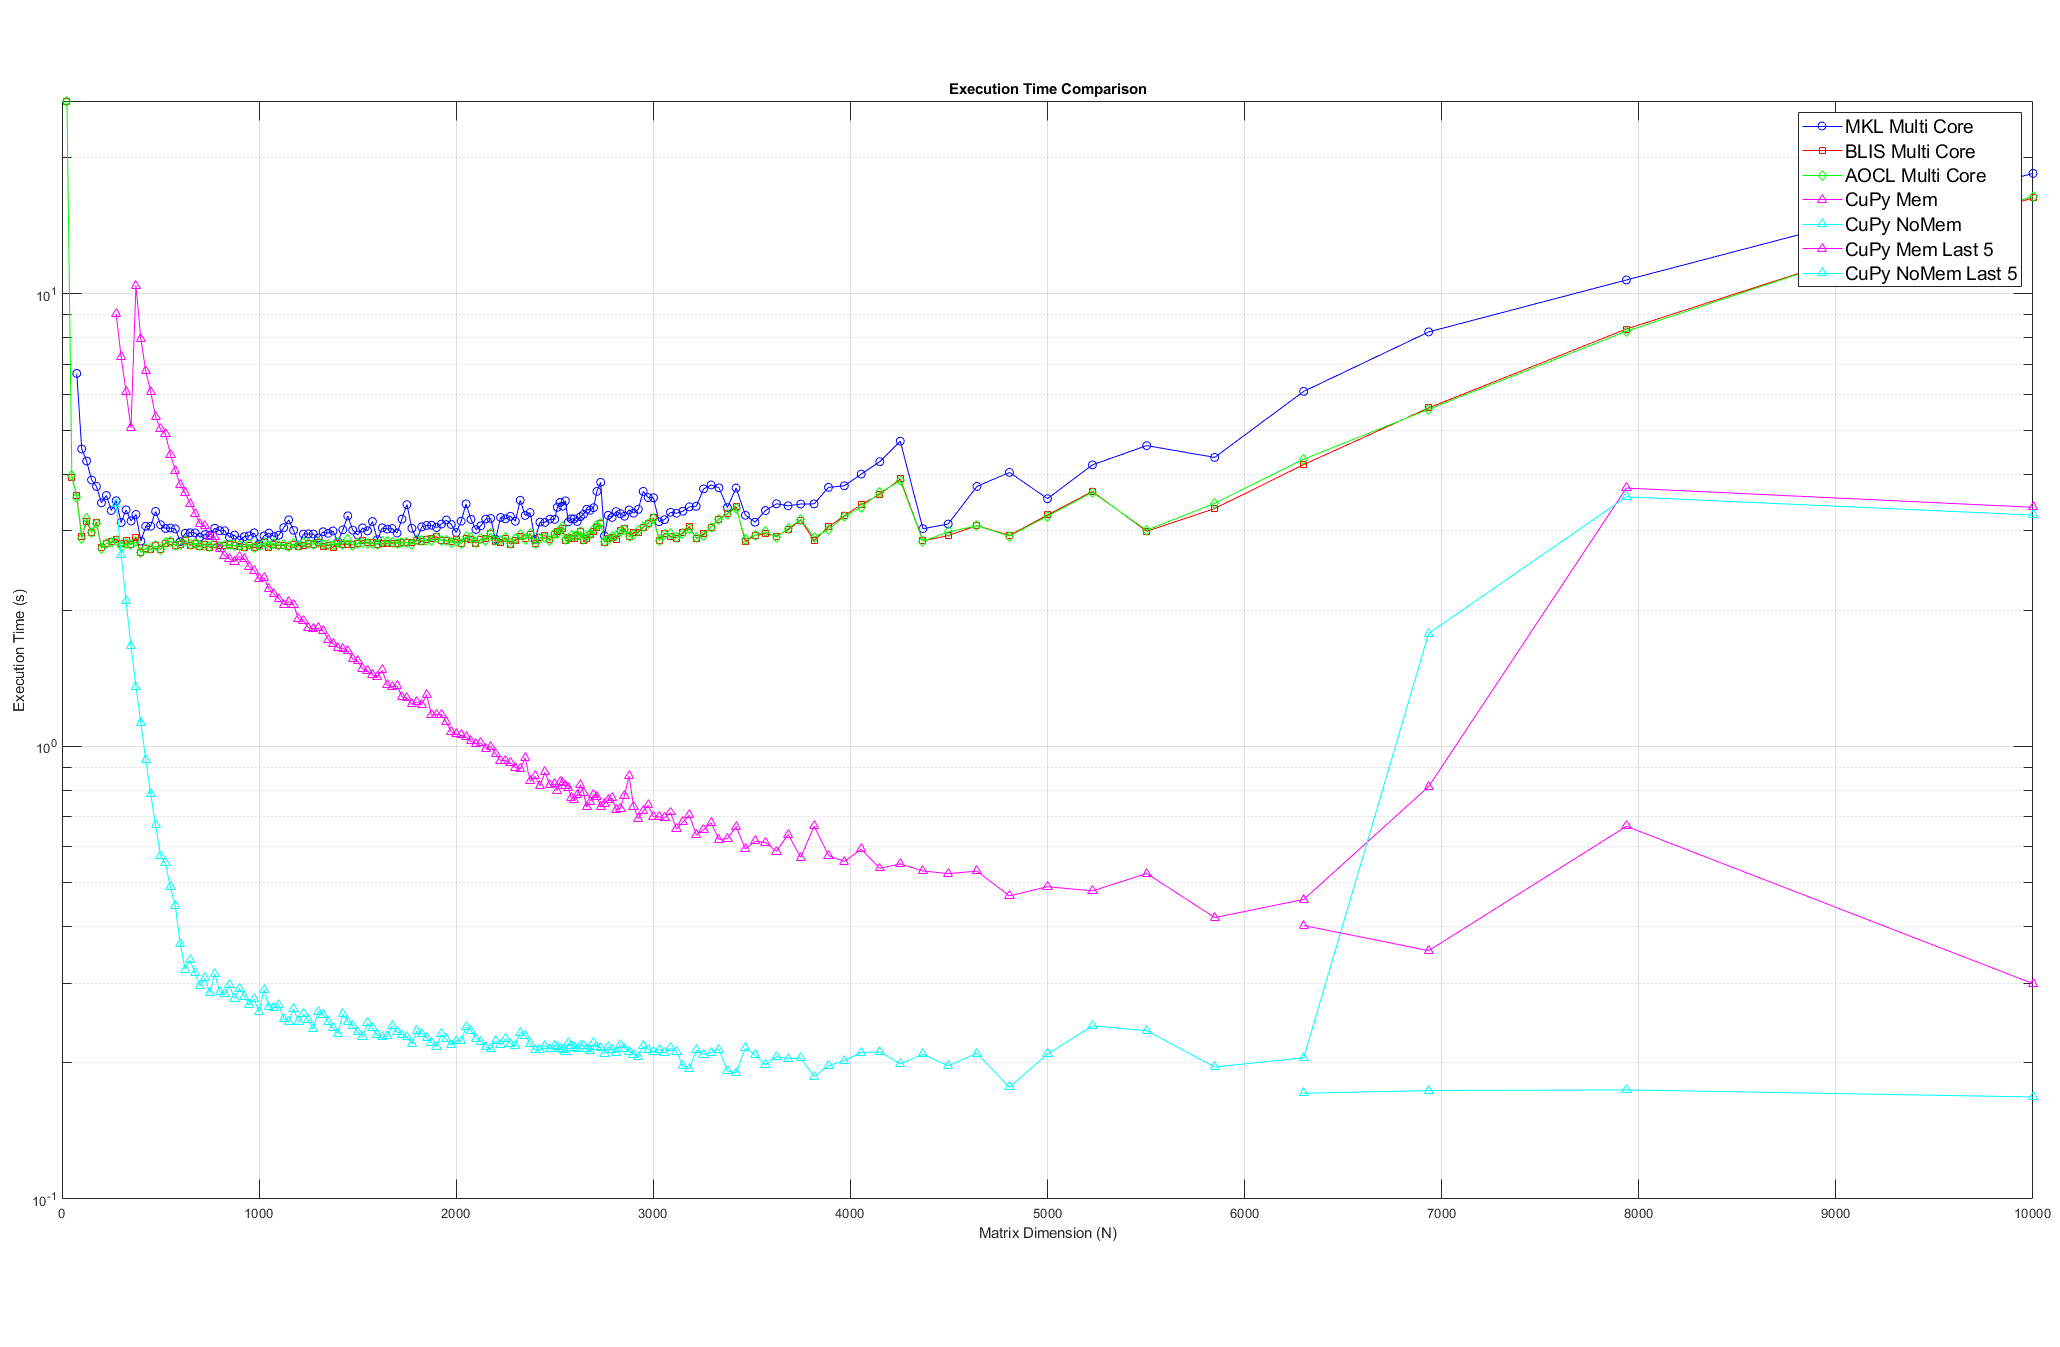
\includegraphics[width=\linewidth]{Figures/Imagenes/Final3.png} % Adjusts the image to the width of the line
\end{figure}

\vspace{-1em}

\textbf{Garbage collector on Python:} The garbage collector impacts CuPy execution times. In the final tests for CuPy, two patterns are observed: one set of results shows increased execution times due to the garbage collector, while the other set, which only includes the last 5 tests, shows improved times without the garbage collector's interference.

\textbf{Memory access:} Even in conditions where memory is copied for every AxB = C operation, GPU performance using CuPy surpasses multi-core CPU implementations by a substantial margin, completing tasks almost an order of magnitude faster.

\subsection{Conclusion}

The analysis highlights the performance differences between multi-core CPU and GPU matrix computation methods. These results are essential for making informed decisions regarding computational methods. Given the GPU's superiority, even under sub-optimal conditions, it suggests a trend towards favoring GPU-based operations in future computational tasks.








\clearpage


%   ---   BIBLIOGRAFÍA/REFERENCIAS   ---   %

%\phantomsection
%\addcontentsline{toc}{section}{Referencias}
%\renewcommand{\refname}{Referencias}
%\bibliographystyle{elsarticle-num}
%\bibliography{references.bib}
%\clearpage



%   ---   ANEXOS   ---   %

%\appendix
%\renewcommand{\appendixname}{Anexos}
%\addcontentsline{toc}{section}{\appendixname}
%\clearpage % or \cleardoublepage
%\appendixpage
%\addappheadtotoc
%\renewcommand{\appendixname}{Anexo}


%\input{./Tex_Files/A_01.tex}
%\clearpage

\end{document}